%%%%%%%%%%%%%%%%%%%%%%%%%%%%%%%%%%%%%%%%%
% Beamer Presentation
% LaTeX Template
% Version 1.0 (10/11/12)
%
% This template has been downloaded from:
% http://www.LaTeXTemplates.com
%
% License:
% CC BY-NC-SA 3.0 (http://creativecommons.org/licenses/by-nc-sa/3.0/)
%
%%%%%%%%%%%%%%%%%%%%%%%%%%%%%%%%%%%%%%%%%

%----------------------------------------------------------------------------------------
%	PACKAGES AND THEMES
%----------------------------------------------------------------------------------------
\documentclass{beamer}

\mode<presentation> {

% The Beamer class comes with a number of default slide themes
% which change the colors and layouts of slides. Below this is a list
% of all the themes, uncomment each in turn to see what they look like.

\usetheme{CambridgeUS}

% As well as themes, the Beamer class has a number of color themes
% for any slide theme. Uncomment each of these in turn to see how it
% changes the colors of your current slide theme.

%\usecolortheme{albatross}
%\usecolortheme{beaver}
%\usecolortheme{beetle}
%\usecolortheme{crane}
%\usecolortheme{dolphin}
%\usecolortheme{dove}
%\usecolortheme{fly}
%\usecolortheme{lily}
%\usecolortheme{orchid}
%\usecolortheme{rose}
%\usecolortheme{seagull}
%\usecolortheme{seahorse}
%\usecolortheme{whale}
%\usecolortheme{wolverine}

%\setbeamertemplate{footline} % To remove the footer line in all slides uncomment this line
%\setbeamertemplate{footline}[page number] % To replace the footer line in all slides with a simple slide count uncomment this line

%\setbeamertemplate{navigation symbols}{} % To remove the navigation symbols from the bottom of all slides uncomment this line
}
%----------------------------------------------------------------------------------------
\usepackage{graphicx} % Allows including images
\usepackage{booktabs} % Allows the use of \toprule, \midrule and \bottomrule in tables
\setbeamerfont{caption}{size=\scriptsize}
\usepackage{hyperref}
\usepackage{listings} % for code listings
\lstset{
  language={C++},
  basicstyle=\footnotesize
}
%----------------------------------------------------------------------------------------
%	TITLE PAGE
%----------------------------------------------------------------------------------------
\title[]{Arduino in der Robotik} % The short title appears at the bottom of every slide, the full title is only on the title page
%----------------------------------------------------------------------------------------
\author{Alexander Entinger} % Your name
\institute{LXRobotics}
\date{\today} % Date, can be changed to a custom date
%----------------------------------------------------------------------------------------
\AtBeginSection{\frame{\sectionpage}}
\AtBeginSubsection{\frame{\subsectionpage}}
%----------------------------------------------------------------------------------------
\begin{document}
%----------------------------------------------------------------------------------------
\begin{frame}
\titlepage % Print the title page as the first slide
\end{frame}
%----------------------------------------------------------------------------------------
%\begin{frame}
\frametitle{Inhalt} % Table of contents slide, comment this block out to remove it
\tableofcontents % Throughout your presentation, if you choose to use \section{} and \subsection{} commands, these will automatically be printed on this slide as an overview of your presentation
%\end{frame}
%%----------------------------------------------------------------------------------------
%%	PRESENTATION SLIDES
%%----------------------------------------------------------------------------------------
\section{Einleitung}
%%----------------------------------------------------------------------------------------
\begin{frame}{Alexander Entinger (1)}
\begin{itemize}
 \item CEO/CTO LXRobotics
  \begin{figure}[H]
   \centering
   
\includegraphics[width=0.3\textwidth]{./images/logo-lxrobotics.png}
   \label{fig:logo-lxrobotics}
  \end{figure}
\end{itemize}
\begin{itemize}
 \item Embedded Software Developer DS Automotion
  \begin{figure}[H]
   \centering
   
\includegraphics[width=0.3\textwidth]{./images/logo-ds-automotion.jpg}
   \label{fig:logo-ds-automotion}
  \end{figure}
\end{itemize}
\begin{itemize}
 \item Projektbetreuer Robotik Fachhochschule Hagenberg
 \begin{itemize}
  \item Masterstudiengang Embedded Systems Design
 \end{itemize}
   \begin{figure}[H]
    \centering
    
\includegraphics[width=0.3\textwidth]{./images/logo-fh-hagenberg.png}
    \label{fig:logo-fh-hagenberg}
   \end{figure}
\end{itemize}
\end{frame}
%%----------------------------------------------------------------------------------------
\begin{frame}{Alexander Entinger (2)}
\begin{columns}
 \begin{column}{0.5\textwidth}
  \begin{large}Mini Sumo Roboter \textbf{Sergeant Pain}\end{large}
  \begin{itemize}
   \item Robotchallenge 2011
  \end{itemize}
 \end{column}
 \begin{column}{0.5\textwidth}
  \begin{figure}[H]
   \centering
   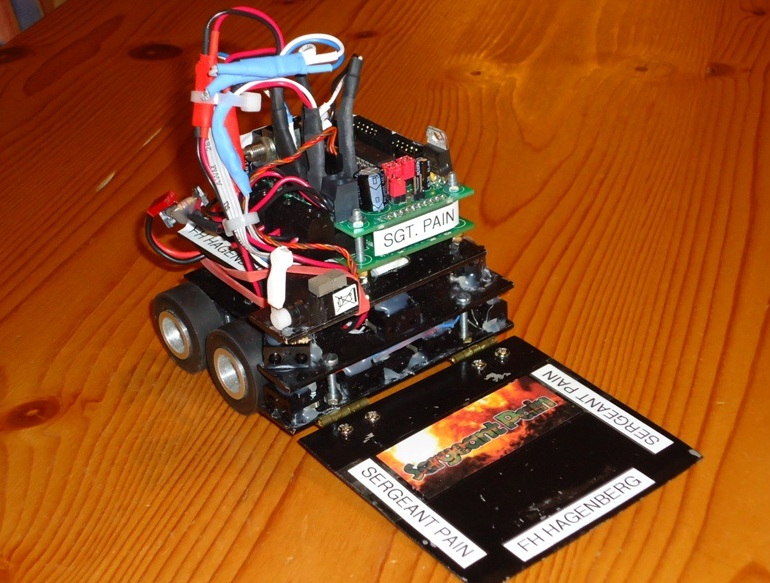
\includegraphics[width=0.7\textwidth]{./images/robot-sergeant-pain.jpg}
   \label{fig:robot-sergeant-pain}
  \end{figure}
 \end{column}
\end{columns}

\begin{columns}
 \begin{column}{0.5\textwidth}
  \begin{large}Mini Sumo Roboter \textbf{Evolution}\end{large}
  \begin{itemize}
   \item Robotchallenge 2014
  \end{itemize}
 \end{column}
 \begin{column}{0.5\textwidth}
  \begin{figure}[H]
   \centering
   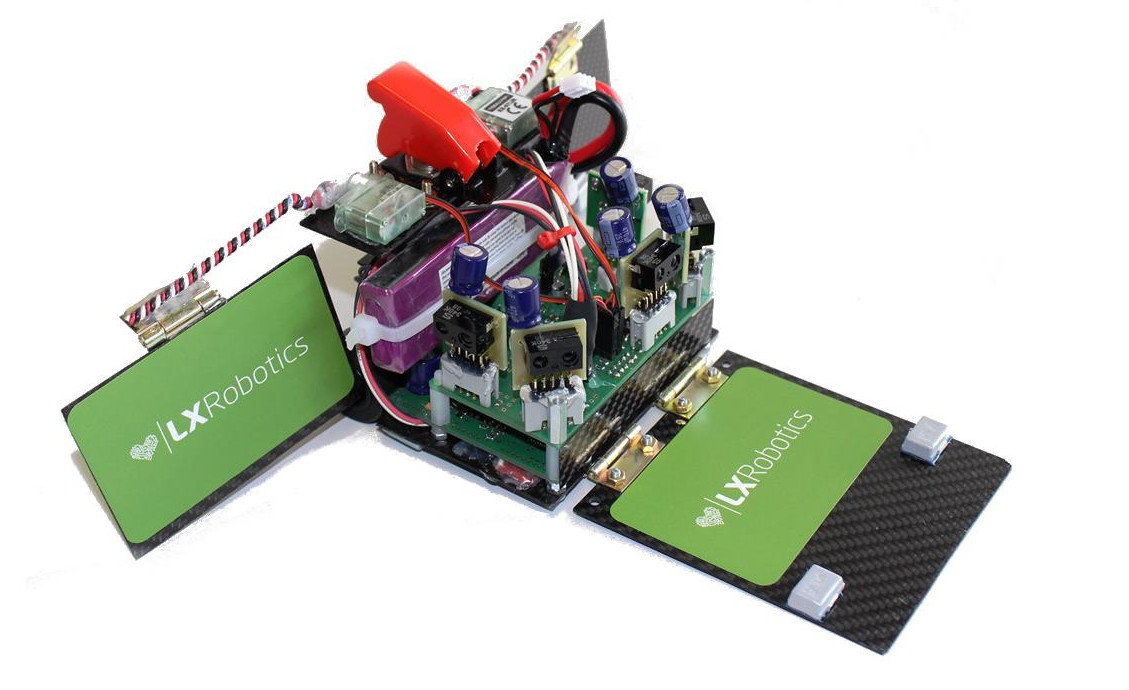
\includegraphics[width=0.7\textwidth]{./images/robot-evolution.jpg}
   \label{fig:robot-evolution}
  \end{figure}
 \end{column}
\end{columns}
\end{frame}
%%----------------------------------------------------------------------------------------
\begin{frame}{Alexander Entinger (3)}
\begin{columns}
 \begin{column}{0.5\textwidth}
  \begin{large}Featherweight \textbf{Schnauzer}\end{large}
  \begin{itemize}
   \item 1. Platz Mad Metal Machines Vol. 19 / Bochum / DE
   \item 1. Platz European Robotcombat Cup 2015
  \end{itemize}
 \end{column}
 \begin{column}{0.5\textwidth}
  \begin{figure}[H]
   \centering
   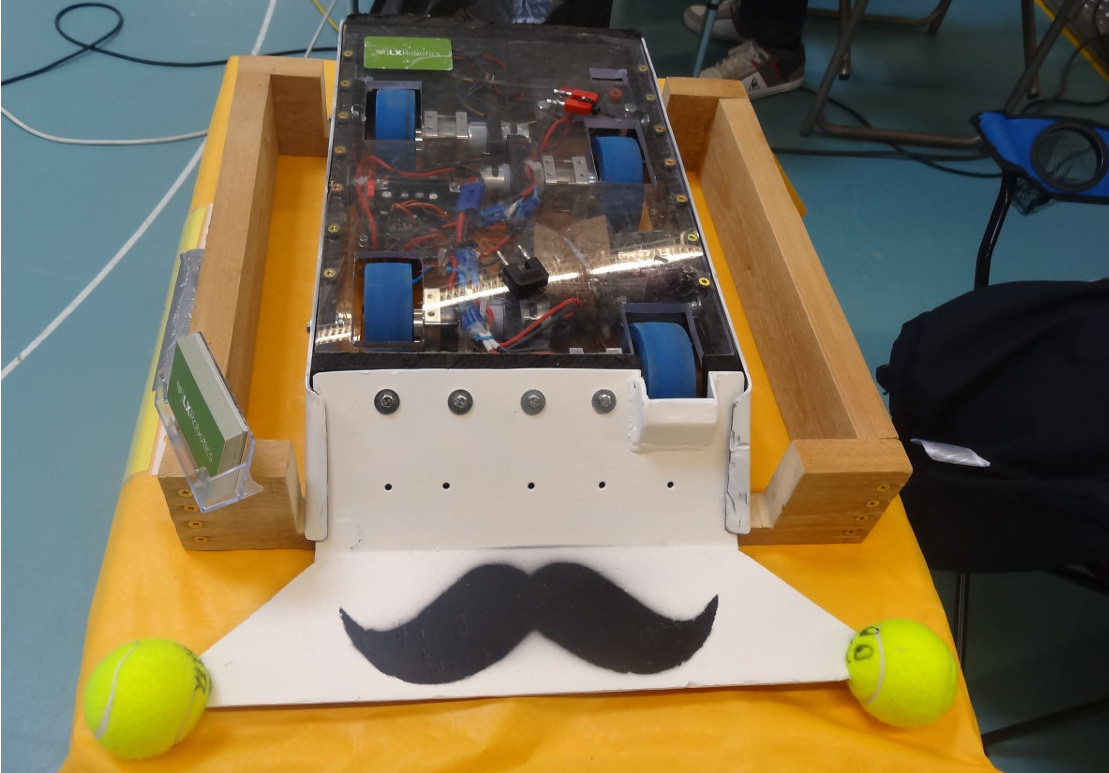
\includegraphics[width=0.7\textwidth]{./images/robot-schnauzer.jpg}
   \label{fig:robot-schnauzer}
  \end{figure}
 \end{column}
\end{columns}

\begin{columns}
 \begin{column}{0.5\textwidth}
  \begin{large}Featherweight \textbf{Steroid}\end{large}
 \end{column}
 \begin{column}{0.5\textwidth}
  \begin{figure}[H]
   \centering
   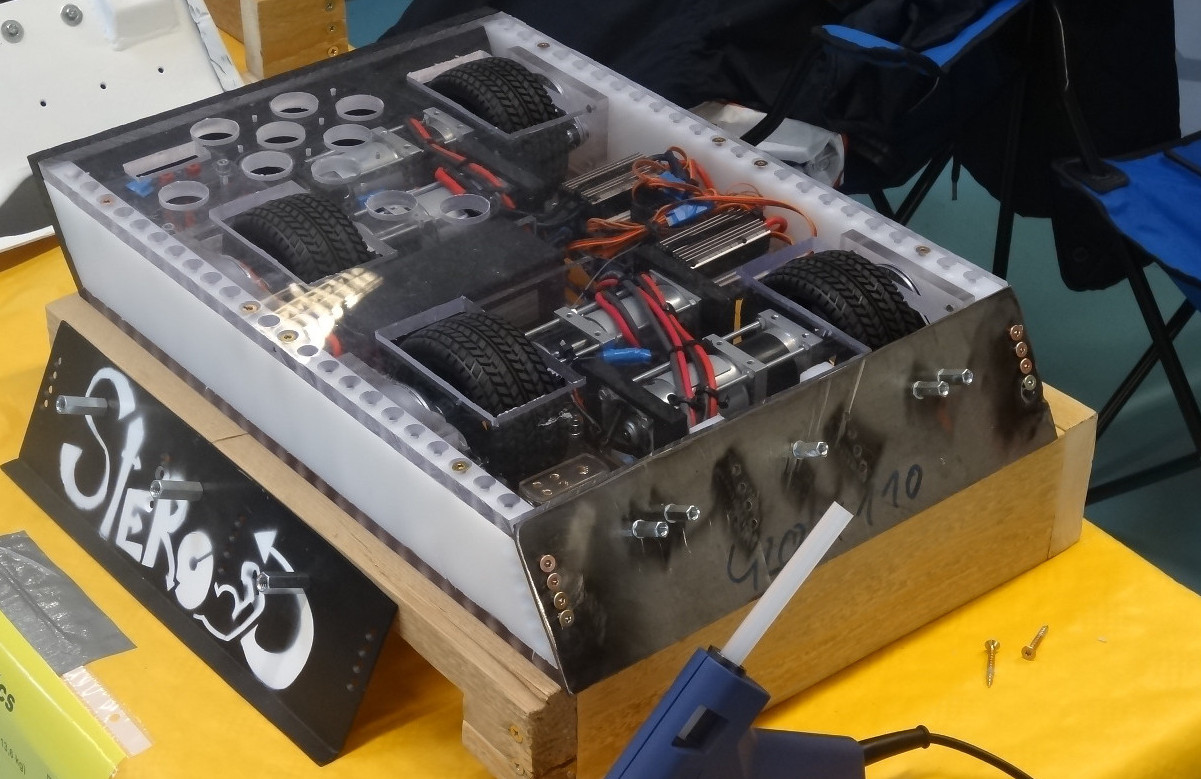
\includegraphics[width=0.7\textwidth]{./images/robot-steroid.jpg}
   \label{fig:robot-steroid}
  \end{figure}
 \end{column}
\end{columns}
\end{frame}
%%----------------------------------------------------------------------------------------
\begin{frame}{Alexander Entinger (4)}
\begin{columns}
 \begin{column}{0.5\textwidth}
  \begin{large}ROS enabled SLAM Demonstrator \textbf{Beauty Queen}\end{large}
  \begin{itemize}
   \item Masterarbeitsprojekt (2012/13)
  \end{itemize}
 \end{column}
 \begin{column}{0.5\textwidth}
 \begin{figure}[H]
  \centering
  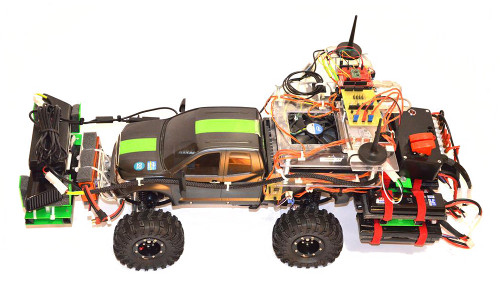
\includegraphics[width=0.7\textwidth]{./images/robot-beauty-queen.jpg}
  \label{fig:robot-beauty-queen}
 \end{figure}
\end{column}
\end{columns}
	
\begin{columns}
 \begin{column}{0.5\textwidth}
  \begin{large}Hexapod \textbf{Lex}\end{large}
 \end{column}
 \begin{column}{0.5\textwidth}
  \begin{figure}[H]
   \centering
   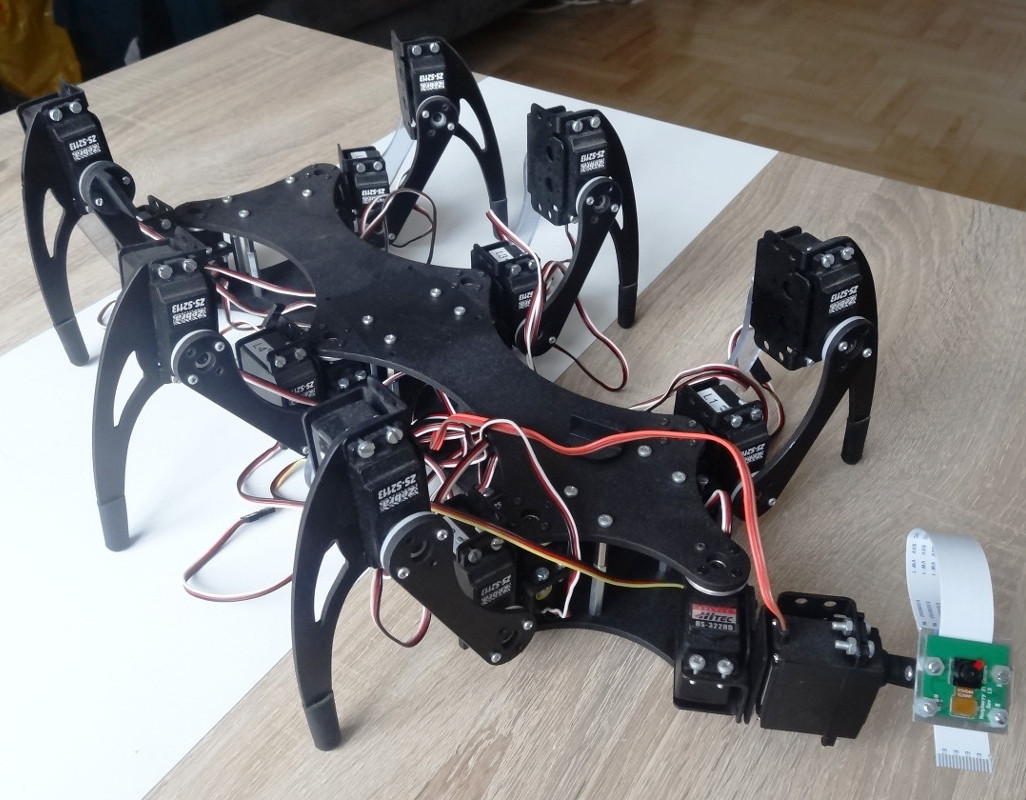
\includegraphics[width=0.7\textwidth]{./images/robot-lex.jpg}
   \label{fig:robot-lex}
  \end{figure}
 \end{column}
\end{columns}

\end{frame}
%%----------------------------------------------------------------------------------------
\section{Was ist eigentlich Arduino?}
%%----------------------------------------------------------------------------------------
\begin{frame}{Arduino}
\begin{large}TODO\end{large}
\end{frame}
%%----------------------------------------------------------------------------------------
\section{Arduino in der Robotik}
%%----------------------------------------------------------------------------------------
\begin{frame}{Sergeant Pain}

\end{frame}
%%----------------------------------------------------------------------------------------
\begin{frame}{Evolution}
	
\end{frame}
%%----------------------------------------------------------------------------------------
\begin{frame}{Schnauzer}
	
\end{frame}
%%----------------------------------------------------------------------------------------
\begin{frame}{Steroid}
	
\end{frame}
%%----------------------------------------------------------------------------------------
\begin{frame}{Beauty Queen}
	
\end{frame}
%%----------------------------------------------------------------------------------------
\begin{frame}{Motivation}
	\begin{itemize}
		\item Die Entwicklung von autonomen Systemen erfordert einen \textbf{enormen Zeitaufwand}
		\begin{itemize}
			\item \textbf{Hardware}, \textbf{Soft}- und \textbf{Firmware}
			\item \textbf{Schnittstellen} und \textbf{Kommunikationsprotokolle} zwischen den zahlreichen Subsystemen
		\end{itemize}
	\end{itemize}
	\begin{itemize}
		\item \textbf{Beobachtung}: Viele Sensoren und Aktoren haben identische Schnittstellen
		\begin{itemize}
			\item IR Distanzsensor/Temperatursenor/Lichtsensor  $\rightarrow$ Analoge Spannung
			\item Ultaschall Distanzsensor/Beschleunigungssensor/Gyroskop $\rightarrow$ I2C
			\item DC Motor, RC Servo Motor $\rightarrow$ PWM
		\end{itemize}
	\end{itemize}
	\begin{itemize}
		\item \textbf{Ziel}: Entwicklung eines I/O-Systems welche die meist verwendeten I/O-Funktionen in \textbf{einem wiederverwendbaren I/O-Modul} integriert
		\begin{itemize}
			\item \textbf{Reduzierung} der f\"ur die Entwicklung eines autonomen Systems ben\"otigte Zeit $\rightarrow$ Das Rad muss nicht immer wieder neu erfunden werden.
		\end{itemize}
	\end{itemize}
\end{frame}
%%----------------------------------------------------------------------------------------
\begin{frame}[fragile]{Implementierung}
	\begin{itemize}
		\item \textbf{Hardware} (Arduino Uno) + \textbf{Software}
		\begin{itemize}
			\item Firmware f\"ur Arduino Uno
			\item C++ Library \textbf{libarduinoio}
		\end{itemize}
		\begin{figure}[htbp]
			\centering
			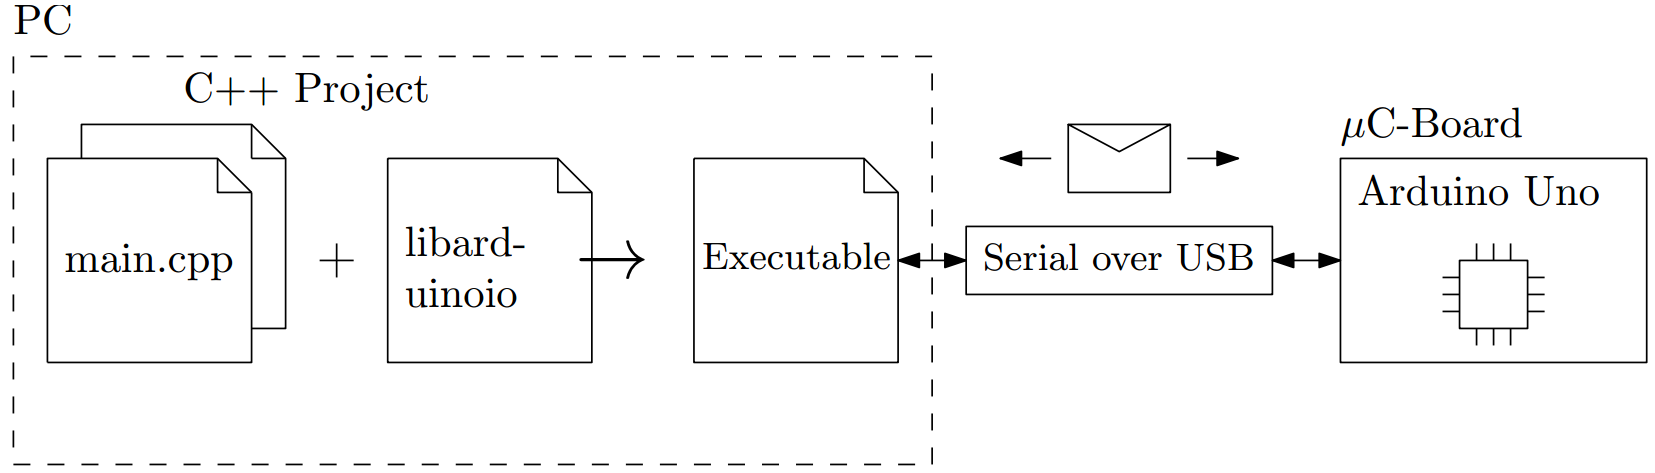
\includegraphics[scale=0.2]{./images/arduinoio-system-overview.png}
		\end{figure}
		\item \textbf{Highlevel Ansteuerung} von $\mu{}C$-I/O-Funktionen
	\end{itemize}
	\begin{lstlisting}
	auto oD2 = io.createGpioOutputPin(arduinoio::D2, false);
	bool const success = oD2->setPinValue(true));
	bool const pin_value = oD2->getPinValue();
	\end{lstlisting}
\end{frame}
%%----------------------------------------------------------------------------------------
\begin{frame}{Leistungsumfang}
	\begin{itemize}
		\item I/O-Funktion verf\"ugbar via $\mu{}C$-I/O-Pin:
		\begin{table}[htbp]
			\begin{tabular}{|c|c|}
				\hline 
				\textbf{I/O-Funktion} & \textbf{Anzahl von I/O-Einheiten} \\ 
				\hline \hline 
				Analoger Eingang & Max. 6 \\ 
				\hline 
				Digitaler Eingang & max. 12  \\ 
				\hline
				Digitaler Ausgang & max. 12 \\ 
				\hline
				Hardware PWM & max. 2 \\ 
				\hline
				Software PWM & max. 6 \\ 
				\hline
				Event Z\"ahler & max. 2 \\
				\hline
				I2C Br\"ucke & max. 1 \\
				\hline
			\end{tabular}
		\end{table}
		\item Weiters:
		\begin{itemize}
			\item Hardware-Reset
			\item 16-Bit Board-ID
			\item Chip-Temperature
		\end{itemize}
	\end{itemize}
\end{frame}
%%----------------------------------------------------------------------------------------
\begin{frame}{Verifikation (1)}
	\begin{itemize}
		\item Die Verifikation der individuellen Komponenten ist nicht zielf\"uhrend $\rightarrow$ Verifikation des Gesamtsystems notwendig
	\end{itemize}
	\begin{itemize}
		\item Gesamtsystem = C++ Library, Kommunikationsschnittstelle, Arduino Firmware $\rightarrow$ \textbf{Ende-Zu-Ende-Verifikation}
	\end{itemize}
	\begin{itemize}
		\item \textbf{Idee}: Einige Pins werden als Eing\"ange, andere als Ausg\"ange definiert und diese auf \textbf{intelligente Art und Weise} miteinander verbunden
	\end{itemize}
	\begin{itemize}
		\item \textbf{Unit Test Framework} f\"ur automatische Ausf\"uhrung aller Tests
	\end{itemize}
\end{frame}
%%----------------------------------------------------------------------------------------
\begin{frame}{Verifikation (2)}
	\begin{itemize}
		\item Digitale Ausg\"ange \textbf{erzeugen} analoge Spannungen via \textbf{R2R Widerstandsnetzwerk}
		\item Analoge Eing\"ange \textbf{messen} diese analogen Spannungen
		\item Testframework \textbf{vergleicht} die gemessene Spannung mit der berechneten Spannung
	\end{itemize}
	\begin{itemize}
		\item 12 digitale Ausg\"ange + 6 analoge Eing\"ange $\rightarrow$ \textbf{6 R2R Widerstandsnetzwerke} mit 2 Bit Aufl\"osung
	\end{itemize}
	\begin{columns}
		\begin{column}{0.4\textwidth}
			\begin{figure}[htbp]
				\centering
				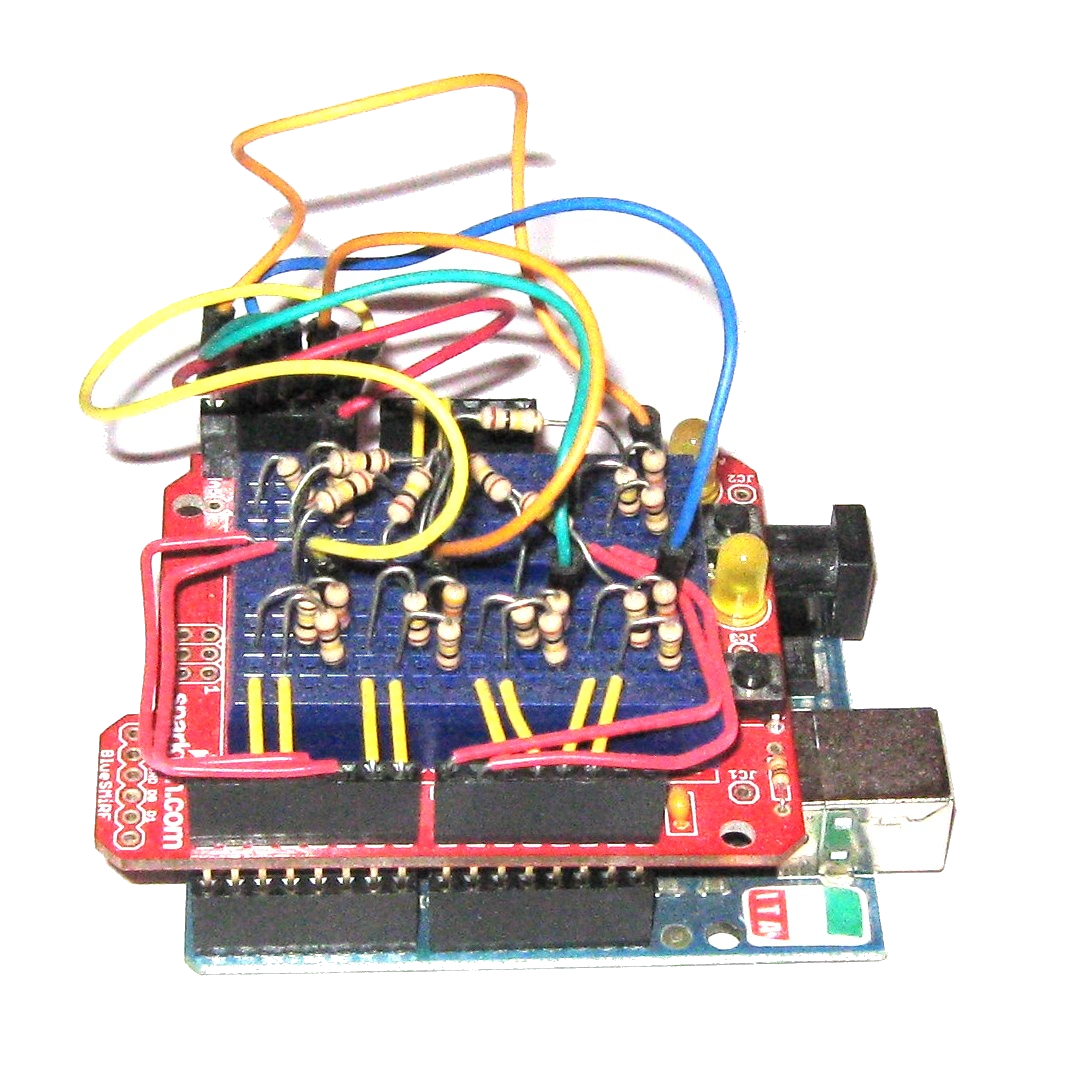
\includegraphics[scale=0.2]{./images/arduinoio-r2r.png}
			\end{figure}
		\end{column}
		\begin{column}{0.4\textwidth}
			\begin{figure}[htbp]
				\centering
				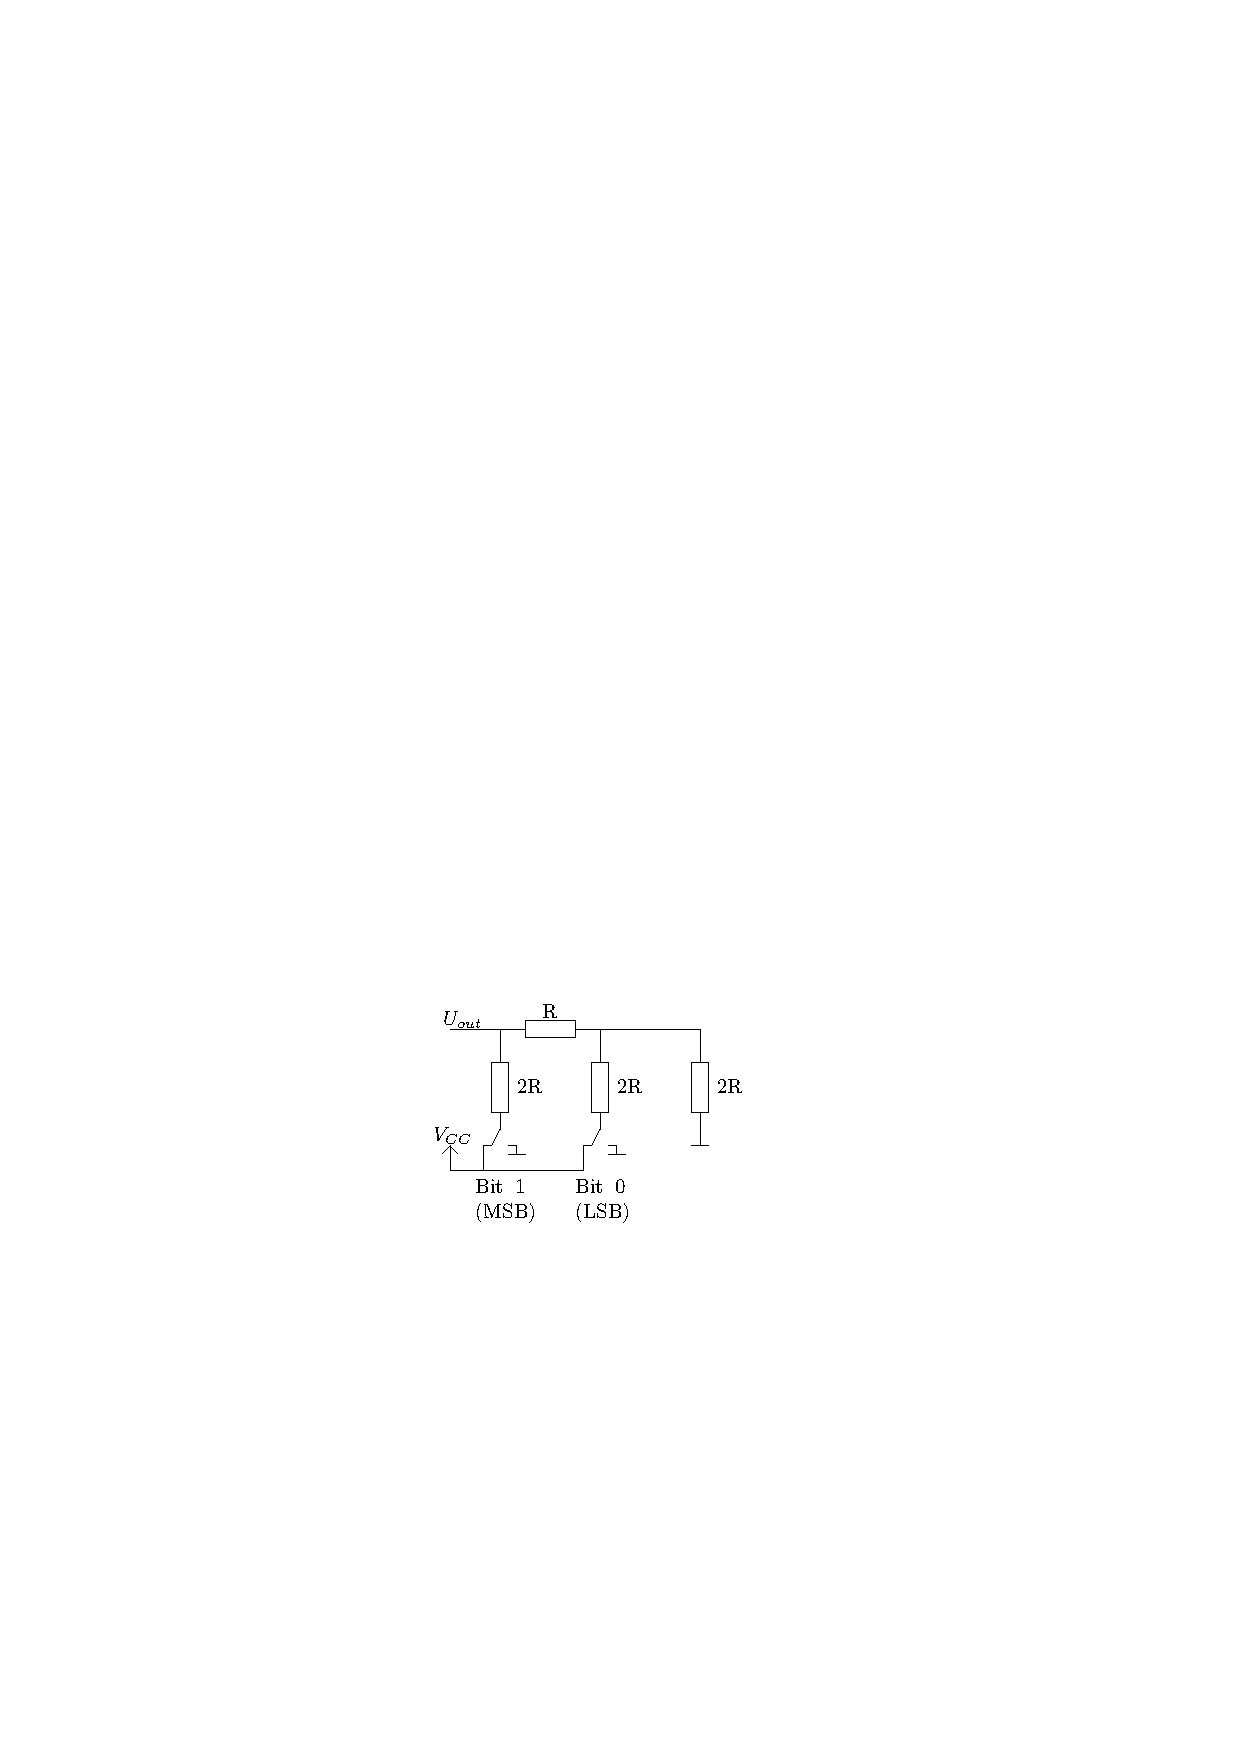
\includegraphics[scale=0.6]{./images/arduinoio-r2r-network.pdf}
			\end{figure}
		\end{column}
	\end{columns}
\end{frame}
%%----------------------------------------------------------------------------------------
\begin{frame}{Command Execution Time}
	\begin{itemize}
		\item \textbf{Command execution time} (CED): Wie lange dauert ein I/O-Befehl?
	\end{itemize}
	\begin{table}[htbp]
		\begin{tabular}{|c|c|}
			\hline 
			\textbf{Command} & \textbf{CED, [CED] = ms} \\ 
			\hline \hline 
			Get ID & 4.15532 ms \\ 
			\hline 
			Set pin value & 4.64086 ms  \\ 
			\hline
			Get pin value & 4.6447 ms \\ 
			\hline
			Get analog value & 5.00152 ms \\ 
			\hline
			I2C Write (1 Byte)  & 4.88282 ms\\ 
			\hline
			I2C Read (1 Byte) & 6.25022 ms \\
			\hline
		\end{tabular}
	\end{table}
	\begin{itemize}
		\item \textbf{Schlussfolgerung}: Hauptanwendungsgebiet sind Applikationen bei denen die CED keine gro\ss{}e Rolle spielt, wie z.B.
		\begin{itemize}
			\item Steuerung von Status LEDs, \"Uberwachen der Batteriespannung, (RC Servo Ansteuerung), etc.
		\end{itemize}
	\end{itemize}
\end{frame}
%%----------------------------------------------------------------------------------------
\begin{frame}{Anwendung in Beauty Queen}
	\begin{itemize}
		\item F\"ur \textbf{Simultaneous Localization and Mapping} (SLAM) modifiziertes RC-Auto
		\item Aufgaben des Arduino-I/O-Systems:
		\begin{columns}
			\begin{column}{0.5\textwidth}
				\begin{itemize}
					\item \textbf{Steuern}
					\begin{itemize}
						\item Electronic Speed Controller
						\item Lenk- und Getriebeservo
						\item Status LEDs
					\end{itemize}
				\end{itemize}
			\end{column}
			\begin{column}{0.5\textwidth}
				\begin{itemize}
					\item \textbf{\"Uberwachen}
					\begin{itemize}
						\item Batteriespannung
					\end{itemize}
				\end{itemize}
			\end{column}
		\end{columns}
		\begin{figure}[htbp]
			\centering
			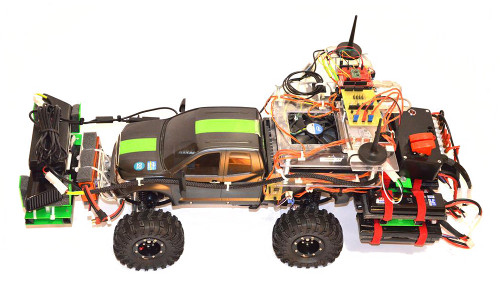
\includegraphics[scale=0.40]{./images/robot-beauty-queen.jpg}
		\end{figure}
	\end{itemize}
\end{frame}
%%----------------------------------------------------------------------------------------
\begin{frame}{Ressourcen}
	\begin{itemize}
		\item Der Quellcodes des Arduino-I/O-Systems steht unter der \textbf{BSD-3}-Lizenz
		\begin{itemize}
			\item Kann f\"ur kommerzielle Applikationen genutzt werden
		\end{itemize}
	\end{itemize}
	\begin{itemize}
		\item \url{https://github.com/lxrobotics/arduinoio}
	\end{itemize}
\end{frame}
%%----------------------------------------------------------------------------------------
\begin{frame}{Lex}
	
\end{frame}
%----------------------------------------------------------------------------------------
\begin{frame}
	\Huge{\centerline{Fragen?}}
\end{frame}
%%----------------------------------------------------------------------------------------
\begin{frame}[allowframebreaks]{References}
%\scriptsize{\bibliographystyle{ieeetr}}
%\bibliography{references} %bibtex file name without .bib extension
\end{frame}
%----------------------------------------------------------------------------------------
\end{document} 
%----------------------------------------------------------------------------------------